\setcounter{chapter}{8}
\setcounter{section}{1}
\setcounter{answer}{0}

\section{Chapter 8: Bayesian statistics}

\answer{
    The prior distribution on the left of the figure assigns equal mass to every value of $\theta$, and therefore does not incorporate relevant information about which values of $\theta$ are more likely to occur. The prior distribution in the middle reflects the belief that the probability of heads is either very close to zero, or very close to one. The prior distribution on the right reflects the information that it is most likely that the coin is a fair coin (highest probability at 0.5), but that there is some uncertainty about $\theta$ around this value.
}

\answer{
        Middle: \hspace*{2.5cm} Right \\
    \\
    $\alpha$: 0.5  \hspace*{2.5cm} $\alpha$: 2
    \answerbreak
    $\beta$: 0.5 \hspace*{2.5cm} $\beta$: 2 \\
    \\
    \answercode{alpha <- 0.5 \\
beta <- 0.5 \\
curve(dbeta(x, alpha, beta), xlab = expression(theta), ylab = \textquotesingle\textquotesingle, yaxt = \textquotesingle n\textquotesingle) \\
\\
alpha <- 2 \\
beta <- 2 \\
curve(dbeta(x, alpha, beta), xlab = expression(theta), ylab = \textquotesingle\textquotesingle, yaxt = \textquotesingle n\textquotesingle)}
}

\answer{
    \hspace*{2.1cm} Biased towards heads: \hspace*{0.65cm} Biased towards tails:
    \vspace*{-7.5pt}
    \begin{center}
        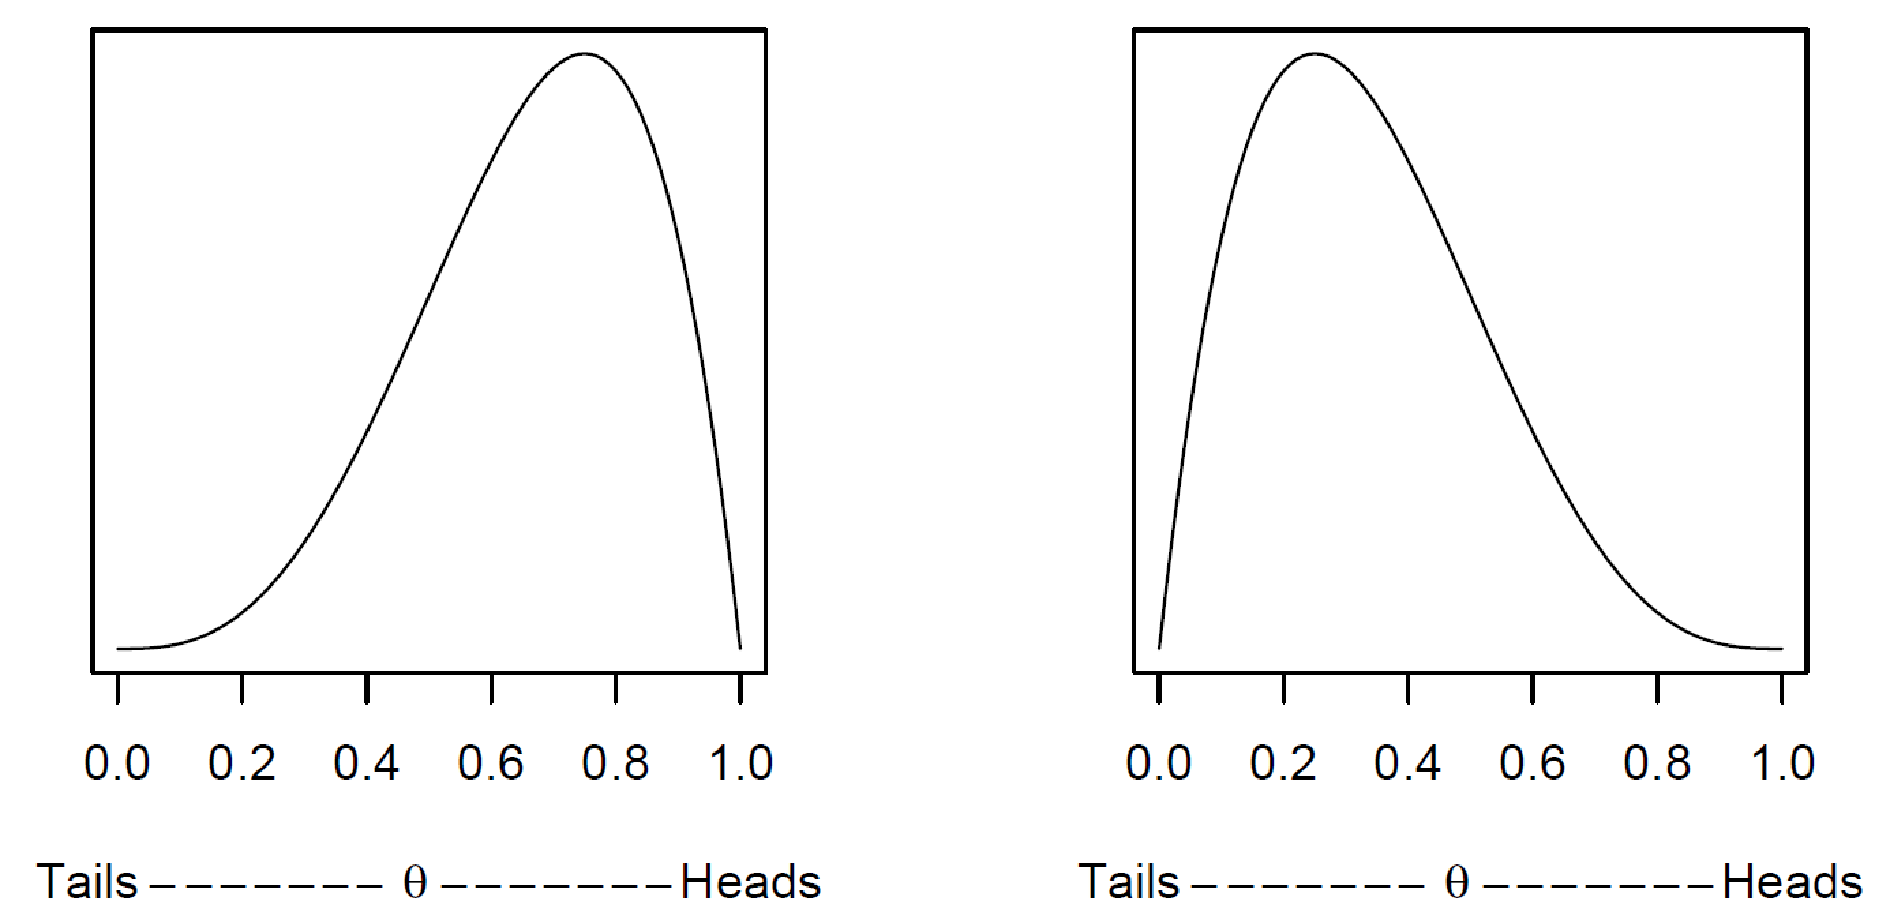
\includegraphics[height=5.3cm]{Files/Images/priorDistributionsAnswer.pdf}
    \end{center}
}

\answerbreakline \setcounter{section}{2} \setcounter{answer}{0}

\answer{
    The Greek letter $\theta$ represents the proportion of customers that leaves the store feeling satisfied in this case.
}

\answer{
    An example of prior parameters can be $\alpha = 7$ and $\beta = 5$. This combination yields a prior distribution that assigns most mass at the point $\theta = 0.6$, but expresses relatively much uncertainty about $\theta$. However, other values of the parameters can also be correct, since the prior reflects your own beliefs. Higher values of $\alpha$ and $\beta$ give prior distributions that are less wide, and this reflect more certain prior beliefs.
}

\clearpage % Page break

\answer{
    The answer depends on your own choices of $\alpha$ and $\beta$ in assignment 8.2b. In the following answers, $alpha = 7$ and $beta = 5$ are used. \\
    \\
    \answercode{curve(dbeta(x, shape1 = 7, shape2 = 5), \\
    \hspace*{35pt}xlab = expression(theta), ylab = \textquotesingle\textquotesingle, yaxt = \textquotesingle n\textquotesingle)}
}

\answer{
    $\alpha$: $7 + 33 = 40$ \hspace*{2cm} $\beta$: $5 + 40 - 33 = 12$
}

\answer{
    Probability: 0.995 \\
    \\
    \answercode{pbeta(0.6, shape1 = 40, shape2 = 12, lower.tail = FALSE) {\color{dataset}\# 0.995}}
}

\answer{
    Probability: 0.875 \\
    \\
    \answercode{diff(pbeta(c(0.7, 0.9), shape1 = 40, shape2 = 12)) {\color{dataset}\# 0.875}}
}

\answer{
    The posterior distribution is fairly robust to changes in the prior distribution. In Bayesian inference, the data quickly overwhelm the prior distribution when it comes to parameter estimation. Therefore, the more data you have the more robust the posterior distribution generally is.
}

\answerbreakline \setcounter{section}{3} \setcounter{answer}{0}

\answer{
    \vspace*{-10pt}
    \answercode{samples <- extract(stanFit)}
}

\answer{
    The histogram approximates the analytical posterior pretty well. The more samples you draw, the better the histogram will resemble the actual posterior distribution. \\
    \\
    \answercode{hist(samples, breaks = 100, probability = TRUE) \\
    curve(dbeta(x, shape1 = 40, shape2 = 12), add = TRUE)}
}

\clearpage % Page break

\answer{
    \vspace*{-10pt}
    \answercode{modelCode <- {\color{dataset}\textquotesingle} \\
{\color{dataset}data \{} \\
    \hspace*{20pt} {\color{dataset}int n;} \\
    \hspace*{20pt} {\color{dataset}int k;} \\
{\color{dataset}\}} \\
{\color{dataset}parameters \{ }\\
    \hspace*{20pt} {\color{dataset}real<lower=0,upper=1> theta; }\\
{\color{dataset}\}} \\
{\color{dataset}model \{ }\\
    \hspace*{20pt} {\color{dataset}theta {\raise.17ex\hbox{$\scriptstyle\sim$}} normal(0.6, 0.1); }\\
    \hspace*{20pt} {\color{dataset}k {\raise.17ex\hbox{$\scriptstyle\sim$}} binomial(n, theta); }\\
{\color{dataset} \} } \\
{\color{dataset}\textquotesingle} \\
\\
{\color{dataset}\# Note: The following line can take a while to execute}\\
compiledModel <- stan\_model(model\_code = modelCode, model\_name = \textquotesingle model\textquotesingle) \\
\\
stanFit <- sampling(compiledModel, data = list(n = 40, k = 33), \\ 
                    \hspace*{110pt}iter = 5000, warmup = 500, chains = 4)}
}

\answer{
    Probability: 0.990 \\
    \\
    \answercode{length(which(samples\$theta > 0.6)) / length(samples\$theta) {\color{dataset}\# 0.990}}
}

\answer{
    Probability: 0.796 \\
    \\
    \answercode{length(which(samples\$theta >= 0.7 \& samples\$theta <= 0.9)) / \\ length(samples\$theta) {\color{dataset}\# 0.796} }
}

\answer{
    The answers of assignments 8.3d and 8.3e do not differ substantially from those of assignments 8.2e and 8.2f. Overall you can conclude that your posterior distribution is fairly robust to changes in the prior distribution. You can therefore be highly sure that the percentage of satisfied customers is higher than 60 percent, and reasonably sure that the percentage lies between 70 and 90 percent.
}

\answerbreakline \setcounter{section}{4} \setcounter{answer}{0}

\answer{
    $H_0$: $\theta = 0.5$ \hspace*{3cm} $H_0$: $\theta \neq 0.5$
}

\answer{
    An example of a possible answer can be $\alpha = 3$ and $\beta = 3$. This prior distribution is fairly wide, and thus expresses not much confidence in your programming skills. \\
    \\
    $\theta \sim Beta(3,\, 3)$
}

\clearpage % Page break

\answer{
    Assuming the values $\alpha = 2$ and $\beta = 2$: \\
    \\
    $\alpha$: 3 + 22 = 25 \hspace*{3cm} $\beta$: 3 + 30 - 22 = 11
}

\answer{
    \vspace*{-10pt}
    \answercode{alpha <- 3 \\
beta <- 3 \\
n <- 30 \\
k <- 22 \\
\\
{\color{dataset}\# Plot the posterior distribution first so no adjustment of the axes is needed}
curve(dbeta(x, alpha + k, beta + n - k), \\
\hspace*{35pt}bty = \textquotesingle n\textquotesingle, las = 1, lty = 1, yaxt = \textquotesingle n\textquotesingle, ylab = \textquotesingle \textquotesingle, xlab = expression(theta)) \\
curve(dbeta(x, alpha, beta), add = TRUE, lty = 2)}
}

\answer{
    \vspace*{-10pt}
    \answercode{heightPrior <- dbeta(0.5, alpha, beta)}
}

\answer{
    \vspace*{-10pt}
    \answercode{heightPosterior <- dbeta(0.5, alpha + k, beta + n - k)}
}

\answer{
    The value of the Bayes factor \rcode{BF10} is 7.02. This implies that the data are 7.18 times more likely to occur under the alternative hypothesis $H_1: \theta \neq 0.5$ than under the null hypothesis $H_0: \theta = 0.5$.
}

\answer{
    The strength of the evidence is moderate, and so you cannot be very confident that your algorithm performs better than change. You will need to collect more data if your want a more decisive Bayes factor.
}

\answerbreakline \setcounter{section}{5} \setcounter{answer}{0}

\clearpage % Page break

\answer{
        $M_1$: $\theta \leq $ 0.75 \hspace{3cm} $M_2$: $\theta \geq$ 0.75
}

\answer{
    \vspace*{-10pt}
    \answercode{model2code <- {\color{dataset}\textquotesingle} \\
{\color{dataset}data \{} \\
    \hspace*{20pt} {\color{dataset}int n;} \\
    \hspace*{20pt} {\color{dataset}int k;} \\
{\color{dataset}\}} \\
{\color{dataset}parameters \{ }\\
    \hspace*{20pt} {\color{dataset}real<lower=0.75,upper=1> theta; }\\
{\color{dataset}\}} \\
{\color{dataset}model \{ }\\
    \hspace*{20pt} {\color{dataset}theta {\raise.17ex\hbox{$\scriptstyle\sim$}} beta(1, 1)T[0.75, 1]; }\\
    \hspace*{20pt} {\color{dataset}k {\raise.17ex\hbox{$\scriptstyle\sim$}} binomial(n, theta); }\\
{\color{dataset} \} } \\
{\color{dataset}\textquotesingle} \\
\\
{\color{dataset}\# Note: The following line can take a while to execute}\\
model2 <- stan\_model(model\_code = model2code, model\_name = \textquotesingle model2\textquotesingle) }
}

\answer{
    The prior distribution for $\theta$ in $M_1$ is a $Beta(1,\, 1)$ prior distribution truncated to the [0, 0.75] interval (\rcode{beta(1, 1)T[0, 0.75]}). The prior distribution for $\theta$ in $M_2$ is a $Beta(1,\, 1)$ prior distribution truncated to the [0.75, 1] interval (\rcode{beta(1, 1)T[0.75, 1]}). 
}

\answer{
    \vspace*{-10pt}
    \answercode{stanFitM1 <- sampling(model1, data = list(n = 156, k = 123), \\ 
                    \hspace*{120pt}iter = 5000, warmup = 500, chains = 4)\\
\\
stanFitM2 <- sampling(model2, data = list(n = 156, k = 123),  \\
                      \hspace*{120pt}iter = 5000, warmup = 500, chains = 4)}
}

\answer{
    \vspace*{-10pt}
    \answercode{mLike1 <- bridge\_sampler(stanFitM1) \\
mLike2 <- bridge\_sampler(stanFitM2)}
}

\answer{
    \vspace*{-10pt}
    \answercode{BF12 <- bf(mLike2, mLike1)}    
}

\answer{
    The value of \rcode{BF12} is around 17.77. This indicates that the data is 17.77 times more likely to occur under model $M_2: \theta \geq 0.75$ than under model $M_2: \theta \leq 0.75$.
}

\answer{
    The evidence in favor of $M_2$ is moderate, and so additional testing might be required to come to a reasonable conclusion.
}

\answerbreakline \setcounter{subsection}{6} \setcounter{answer}{0}

\clearpage % Page break

\answer{
    \vspace*{-10pt}
    \answercode{{\color{dataset}\# Be sure to set your working directory when providing a relative path} \\
insurance <- read.csv(\textquotesingle insurance.csv\textquotesingle)}
}

\answer{
    charges = $\beta_0\, + \,\beta_1\,\, \times $ age $+ \,\beta_2\,\, \times $ bmi $+\, \beta_3\,\, \times $ neighbors 
}

\answer{
    $\beta_0$: -6670.25 \hspace*{1cm} $\beta_1$: 333.92 \hspace*{1cm} $\beta_2$: 241.56 \hspace*{1cm} $\beta_3$: 45.84 \\
    \\
    \answercode{regressionFit <- sampling(object = regressionModel, \\
    \hspace*{165pt}data = list(N = nrow(insurance), \\
        \hspace*{230pt}x1 = insurance\$bmi, \\
        \hspace*{230pt}x2 = insurance\$age, \\
        \hspace*{230pt}x3 = insurance\$neighbors, \\
        \hspace*{230pt}y = insurance\$charges),\\
        \hspace*{165pt}iter = 5000, warmup = 500, chains = 4) \\
                        \\
                        regressionSamples <- extract(regressionFit) \\
                        summary(regressionSamples)}
}

\answer{
    YES \\
    \\
    \answercode{summary(lm(charges {\raise.17ex\hbox{$\scriptstyle\sim$}} 1 + age + bmi + neighbors, data = insurance))}
}

\answer{
    \vspace*{-10pt}
    \answercode{layout(matrix(1:4, nrow = 2)) \\
    \\
    plot(density(regressionSamples\$beta1), xlab = \textquotesingle \textquotesingle, ylab = \textquotesingle \textquotesingle, \\
\hspace*{30pt}yaxt = \textquotesingle n\textquotesingle, bty = \textquotesingle n\textquotesingle, main = expression(beta[1])) \\
plot(density(regressionSamples\$beta0), xlab = \textquotesingle \textquotesingle, ylab = \textquotesingle \textquotesingle, \\
\hspace*{30pt}yaxt = \textquotesingle n\textquotesingle, bty = \textquotesingle n\textquotesingle, main = expression(beta[0])) \\
plot(density(regressionSamples\$beta2), xlab = \textquotesingle \textquotesingle, ylab = \textquotesingle \textquotesingle, \\
\hspace*{30pt}yaxt = \textquotesingle n\textquotesingle, bty = \textquotesingle n\textquotesingle, main = expression(beta[2])) \\
plot(density(regressionSamples\$beta3), xlab = \textquotesingle \textquotesingle, ylab = \textquotesingle \textquotesingle, \\
\hspace*{30pt}yaxt = \textquotesingle n\textquotesingle, bty = \textquotesingle n\textquotesingle, main = expression(beta[3])) \\
\\
layout(1)}
}

\answer{
    Probability: 0.966\\
    \\
    \answercode{length(which(regressionSamples\$beta2 > 200)) / length(regressionSamples\$beta2)}
}

\clearpage % Page break

\answer{
    Probability: 0.052\\
    \\
    \answercode{length(which(regressionSamples\$beta1 < 250)) / length(regressionSamples\$beta1)}
}

\answer{
    Lower bound: -79.98 \hspace*{3cm} Upper bound: 169.74 \\
    \\
    \answercode{quantile(regressionSamples\$beta3, probs = c(0.10, 0.90))}
}

\answer{
    \vspace*{-10pt}
    \answercode{regressionmodelcode2 <- {\color{dataset}\textquotesingle} \\
{\color{dataset}data \{} \\
    \hspace*{20pt} {\color{dataset}int<lower=0> N;} \\
    \hspace*{20pt} {\color{dataset}vector[N] x1;} \\
    \hspace*{20pt} {\color{dataset}vector[N] x2;} \\
    \hspace*{20pt} {\color{dataset}vector[N] y;} \\
{\color{dataset}\}} \\
{\color{dataset}parameters \{ }\\
    \hspace*{20pt} {\color{dataset}real beta0; }\\
    \hspace*{20pt} {\color{dataset}real beta1; }\\
    \hspace*{20pt} {\color{dataset}real beta2; }\\
    \hspace*{20pt} {\color{dataset}real<lower=0> sigma; }\\
{\color{dataset}\}} \\
{\color{dataset}model \{ }\\
    \hspace*{20pt} {\color{dataset}y {\raise.17ex\hbox{$\scriptstyle\sim$}} normal(beta0 + beta1 * x1 + beta2 * x2, sigma);}\\
{\color{dataset} \} } \\
{\color{dataset}\textquotesingle} \\
\\
{\color{dataset}\# Note: The following line can take a while to execute}\\
regressionModel2 <- stan\_model(model\_code = regressionmodelcode2,  \\ 
\hspace*{150pt}model\_name = \textquotesingle Regression2\textquotesingle) }
}

\answer{
    \vspace*{-10pt}
    \answercode{regressionFit2 <- sampling(object = regressionModel2, \\
    \hspace*{165pt}data = list(N = nrow(insurance), \\
        \hspace*{230pt}x1 = insurance\$bmi, \\
        \hspace*{230pt}x2 = insurance\$age, \\
        \hspace*{230pt}y = insurance\$charges),\\
        \hspace*{165pt}iter = 5000, warmup = 500, chains = 4) \\
                        \\
                        mLike1 <- bridge\_sampler(regressionFit) \\
                        mLike2 <- bridge\_sampler(regressionFit2) \\
                        \\
                        BF12 <- bf(mLike1, mLike2)}
}

\clearpage % Page break

\answer{
    The value of \rcode{BF12} is 258.65. This implies that the data are 258.65 times as likely to be observed under the model where $\beta_3$ is not included in the regression equation under the model where $\beta_3$ is included. The evidence against the number of \rcode{neighbors} adding to the prediction accuracy is extreme.
}

\clearpage % Page break